\documentclass[
% twocolumn,
% hf,
]{ceurart}

%% One can fix some overfulls
\sloppy

%% Minted listings support 
%% Need pygment <http://pygments.org/> <http://pypi.python.org/pypi/Pygments>
\usepackage{listings}
\usepackage{pgfplots}
\pgfplotsset{compat=1.18}
\usepackage{tikz}
\usetikzlibrary{shapes.geometric, arrows.meta, positioning, fit, calc, backgrounds}
%% auto break lines
\lstdefinelanguage{json}{
  basicstyle=\small\ttfamily,
  columns=fullflexible,
  showstringspaces=false,
  breaklines=true,
}
\lstset{breaklines=true}


\begin{document}

%% Rights management information.
%% CC-BY is default license.
\copyrightyear{2026}
\copyrightclause{Copyright for this paper by its authors.
  Use permitted under Creative Commons License Attribution 4.0
  International (CC BY 4.0).}

%% This command is for the conference information
\conference{ITAT 2026: Information Technologies -- Applications and Theory, September 25--29, 2026, Hotel Vršatec, Slovakia}

\title{Hybrid Context-Aware Access Control for IoT Devices Using Multi-Agent LLMs: A Security Evaluation}

\author[1]{Ahmed Fouad Lagha}[%
email=ahmed.lagha@inf.elte.hu,
orcid=0009-0005-8255-9434,
]
\cormark[1]
\author[1]{Loubna Seddiki}[%
email=seddikiloubna@inf.elte.hu,
orcid=0009-0006-7209-6138,
]
\author[1]{Oumaima Araar}[%
email=oumaima.araar@inf.elte.hu,
]
\author[1]{Imre Lendák}[%
email=lendak@inf.elte.hu,
orcid=0000-0001-6188-4936,
]

\address[1]{Department of Data Science and Engineering, Eötvös Loránd University, Budapest, Hungary}

\cortext[1]{Corresponding author.}

\begin{abstract}
    Traditional Role-Based Access Control (RBAC) is too rigid to adapt to dynamic IoT threats. We propose IoT-Access-Sentinel, a hybrid framework that combines deterministic validation with Large Language Model (LLM) reasoning for context-aware access control. On a synthetic benchmark, the LLM layer alone was vulnerable to prompt injection. However, pairing a hardened deterministic pre-filter with strict semantic delimiters substantially improved robustness in this benchmark. Integrated with the Wazuh SIEM~\cite{wazuh2024}, IoT-Access-Sentinel shows that LLMs can support complex access policies when they are anchored by strict input sanitization.
\end{abstract}

\begin{keywords}
    IoT Security \sep Access Control \sep Large Language Models \sep Multi-Agent Systems \sep Adversarial Testing \sep SIEM Integration
\end{keywords}

\maketitle

\section{Introduction}

The proliferation of Internet of Things (IoT) devices in critical infrastructure, smart homes, and industrial environments has created new security challenges for access control. As devices move from isolated components to interconnected ecosystems, authorization decisions must account not only for identity and policy rules, but also for context such as time, device state, user intent, and operational environment. Traditional approaches such as Role-Based Access Control (RBAC) remain effective for deterministic enforcement, but they are often too rigid to resolve semantic ambiguity in dynamic IoT settings.

Recent generative-AI work in IoT security has largely focused on offline policy generation or passive detection, leaving a gap in runtime access management. In particular, real-time authorization remains difficult because conventional rule engines struggle with natural-language or context-heavy requests, while unconstrained LLM reasoning is vulnerable to prompt injection and other adversarial manipulations. As a result, systems that are expressive enough to reason about context may also be too fragile to trust directly in the authorization path.

We address this gap with \textit{IoT-Access-Sentinel}, a hybrid framework that places deterministic validation and multi-agent LLM reasoning in a single access-control pipeline. The system first applies strict security-critical checks, including token validation and user-device mapping, and only then uses specialized LLM agents to resolve ambiguous cases. The resulting design keeps the enforcement boundary deterministic while using the LLM layer where semantic reasoning is most useful.

We evaluate the framework on a synthetic benchmark of benign and adversarial scenarios. The results show that the LLM layer alone is vulnerable to prompt injection, but that combining it with a hardened deterministic pre-filter and strict prompt delimiting substantially improves robustness in this benchmark. Our findings suggest that LLMs can support runtime access control for IoT systems, provided they operate inside a narrow containment boundary with fail-secure defaults.

This study makes the following contributions.

\begin{itemize}
    \item \textbf{Hybrid access-control architecture.} We propose a two-stage IoT authorization pipeline that combines deterministic validation with multi-agent LLM reasoning for context-aware decision-making.

    \item \textbf{Security-focused evaluation.} We assess the approach on a synthetic benchmark with benign and adversarial scenarios, showing both the benefits and the attack surface of LLM-assisted authorization.

    \item \textbf{Defense-in-depth and reproducibility.} We show how deterministic sanitization, prompt delimiters, and fail-secure behavior reduce structural and semantic attacks, and we release the codebase, benchmark scenarios, and analysis scripts for reproducibility.
\end{itemize}

The remainder of this paper is organized as follows. Section~\ref{sec:related_work} reviews prior work on LLM-based and traditional access control, including a comparison table that summarizes how our system differs from prior LLM-based access-control approaches. Section~\ref{sec:adversarial_eval} presents the threat model and adversarial evaluation, Section~\ref{sec:decision_pipeline} describes the system architecture, and the remaining sections report the experimental results, limitations, and future directions.

\section{Related Work}\label{sec:related_work}

\subsection{LLM-based Access Control for IoT}

Recent studies have explored large language models for IoT access control~\cite{llm4iot2024, edgegenai2024}, primarily focusing on policy generation from natural language specifications.

LACE~\cite{lace2025} introduces a Language-based Access Control Engine that translates natural language policy descriptions into structured rules. LACE combines LLM-based policy generation with formal verification using an Open Policy Agent (OPA) and reports 88\% runtime decision accuracy. It illustrates one approach to coupling LLMs with policy enforcement, but its LLM-assisted decision pathway adds runtime latency (2.66s per request) that may limit use in time-sensitive settings.

CollabIoT~\cite{shastri2025llmdrivenautoconfigurationtransient} employs LLM-driven capability-based access control for transient IoT collaboration. The system focuses on policy generation and device auto-configuration, reporting validated access control policies with 100\% correctness and low enforcement overhead. CollabIoT is therefore best viewed as a complementary approach: it emphasizes proactive token generation, whereas our work examines reactive runtime authorization when requests are semantically ambiguous.

Taken together, LACE and CollabIoT show how LLMs can support policy creation and configuration. Our system instead explores real-time access decisions on alerts, using multi-agent LLM reasoning only when deterministic validation cannot resolve the semantic ambiguity. Table~\ref{tab:related_comparison} summarizes these differences.

\begin{table}[h]
    \centering
    \caption{Comparison with LLM-based IoT Access Control Systems}
    \label{tab:related_comparison}
    \begin{tabular}{lccc}
        \toprule
        \textbf{System}                & \textbf{LLM Role} & \textbf{Decision Time} & \textbf{Accuracy} \\
        \midrule
        LACE~\cite{lace2025}           & Policy \& Decisions & Runtime (2.66s)       & 88\% (runtime)    \\
        CollabIoT~\cite{shastri2025llmdrivenautoconfigurationtransient} & Policy generation & Offline (7.07--22.41s) & 100\% (policy)    \\
        \textbf{Ours (Hybrid)}         & Runtime decisions & Real-time (97ms)       & 94.1\% (runtime)  \\
        \bottomrule
    \end{tabular}
\end{table}

\subsection{Traditional Access Control for IoT}

Traditional IoT access control relies on static rule-based approaches, such as RBAC~\cite{rbac2004}, ABAC~\cite{abac2012}, and capability-based systems~\cite{capability2016}. These methods excel at deterministic validation but struggle with semantic threats and contextual anomalies~\cite{alaba2017internet, ouaddah2016fairaccess}.

DLBAC~\cite{dlbac2022} proposes deep-learning-based access control using neural networks to learn access patterns. While improving static RBAC, DLBAC lacks explainability, which is critical for M0801 compliance, where security decisions must be auditable.

RASA~\cite{rasa2021} introduces risk-aware adaptive access control using Bayesian networks. However, RASA's risk scores lack semantic transparency, making it difficult for security operators to answer the question of ``why'' a request was denied, which is a critical requirement for post-incident auditing and M0801 compliance.

Multi-agent LLM frameworks~\cite{multiagent2023} have shown that specialized agents can outperform monolithic general-purpose models on structured tasks. IoT-Access-Sentinel follows this pattern by separating context extraction from policy evaluation. This design is consistent with recent risk-management and secure-agent work, including the NIST AI RMF~\cite{nist_airmf_2023} and CaMeL~\cite{camel2024}, which emphasize capability separation and deterministic containment.


\subsection{LLM Vulnerabilities in Cyber-Physical Systems}

Recent literature on Natural Language Access Control (NLAC)~\cite{lace2025, xu2022building} explores the translation of user intent into formal access policies. These systems typically use LLMs for policy \textit{generation} (intent $\rightarrow$ rule), whereas IoT-Access-Sentinel uses LLMs for \textit{runtime evaluation} (rule + context $\rightarrow$ decision). This runtime delegation introduces risks that have been documented in prior work on AIoT and agentic systems: prompt injection can manipulate model outputs, and adversarial techniques such as jailbreaking and payload splitting can bypass standard alignment guardrails~\cite{yao2024survey, agentsec2025, wei2023jailbroken, liu2024autodan, fang2024llm}. These observations motivate the deterministic containment boundary (Layer 0) used in our architecture~\cite{doshi2024llms}.

\section{Threat Model and Adversarial Robustness}

\subsection{Threat Model}

Our system operates under an adversarial threat model in which attackers may attempt to bypass access control through input manipulation, prompt injection, SQL injection, Unicode-based obfuscation, semantic evasion, or network/time bypasses. We assume that attackers can observe the system architecture, adapt their payloads over time, and interact with the IoT network, but they do not possess valid authentication credentials.

\subsection{Defense Mechanisms}

The hybrid architecture implements a two-layer defense pipeline. Layer 0 performs deterministic validation before any LLM reasoning occurs. It combines schema validation for incoming alerts, security-critical authentication checks, and pattern matching for obvious injection attempts, and it defaults to DENY when credentials are missing or malformed. Layer 1 handles only the requests that survive Layer 0. It uses zero-trust prompts, structured JSON outputs, and agent separation to reduce prompt leakage and attack propagation, while allowing the Context and Policy agents to reason about more subtle semantic attacks and generate auditable explanations.

\subsection{Adversarial Evaluation}\label{sec:adversarial_eval}

We evaluated the robustness against 105 diverse red-team scenarios spanning 10 distinct attack categories to ensure comprehensive coverage of the adversarial space:

\begin{table}[h]
    \centering
    \caption{Adversarial Attack Detection Results (105 Scenarios)}
    \label{tab:adversarial}
    \begin{tabular}{lcc}
        \toprule
        \textbf{Attack Category} & \textbf{Tested} & \textbf{Detected}   \\
        \midrule
        Direct Prompt Injection  & 10              & 10 (100\%)          \\
        Role-Play Hijack         & 10              & 10 (100\%)          \\
        Unicode RTLO/Evasion     & 10              & 10 (100\%)          \\
        Hidden Char Evasion      & 10              & 10 (100\%)          \\
        Payload Splitting        & 10              & 10 (100\%)          \\
        Semantic Deception       & 5               & 5 (100\%)           \\
        Chain-of-Thought Hijack  & 10              & 10 (100\%)          \\
        Contextual Contradiction & 10              & 10 (100\%)          \\
        Advanced Injection       & 15              & 15 (100\%)          \\
        Metadata Smuggling       & 15              & 15 (100\%)          \\
        \midrule
        \textbf{Overall}         & \textbf{105}    & \textbf{105 (100\%)} \\
        \bottomrule
    \end{tabular}
\end{table}

The deterministic validator detected 66.7\% of adversarial attempts (70/105) in Layer 0 before reaching the LLM agents. The implementation used Unicode NFKC normalization, invisible-character stripping, and regex-based blocklists. These mitigations convert obfuscated payloads (for example, RTLO characters or zero-width smuggling) into canonical forms, allowing Layer 0 to trigger immediate DENY decisions. The remaining 33.3\% of attacks (35/105)—primarily involving contextual contradiction, CoT hijacking attempts, and metadata smuggling—were handled by the Policy Agent's contextual reasoning and fail-secure logic.

To address the concern of ``ceding enforcement to the LLM'', we use Layer 0 (Deterministic Validator) as a containment boundary. Every field is processed through a \texttt{normalize\_text} method using \texttt{unicodedata.normalize('NFKC')} to resolve homoglyph attacks, followed by regex stripping of \textbf{directional overrides} (\texttt{\textbackslash u202A-\textbackslash u202E}), \textbf{Bidi Isolates} (\texttt{\textbackslash u2066-\textbackslash u2069}), and zero-width control characters. Unlike LACE's formal OPA check, which occurs \textit{after} policy generation, our sentinel's formal checks occur \textit{before} the LLM sees the data, ensuring that the LLM reasons only on sanitized, canonicalized context. For the 46\% of requests handled by Layer 0, the LLM was bypassed. On the remaining 54\% of ``semantically ambiguous'' cases, our multi-agent chain (Layer 2/3) provides a 6.1 percentage point accuracy lift over the 88\% accuracy benchmark reported by policy-generation-only systems such as LACE.


\section{System Architecture}

The IoT-Access-Sentinel follows an Observe $\rightarrow$ Decide $\rightarrow$ Act pipeline. Figure~\ref{fig:architecture} summarizes the flow from log ingestion to enforcement. The Observe stage collects security-relevant events from Wazuh, the Decide stage applies deterministic checks and LLM-based reasoning, and the Act stage translates authorization outcomes into distributed enforcement.

\begin{figure}[ht]
    \centering
    \includegraphics[width=0.9\textwidth]{architecture.pdf}
    \caption{IoT-Access-Sentinel Architecture Pipeline. Layer 0 applies deterministic validation, and Layer 1 performs semantic reasoning on ambiguous alerts.}
    \label{fig:architecture}
\end{figure}

\subsection{Observe: Wazuh SIEM Integration}

We deployed custom decoders and rules in the Wazuh Manager~\cite{wazuh2024} to parse IoT access logs and classify events by device type, including cameras, sensors, and smart locks. The rules cover network violations, temporal violations, unknown device attempts, and high-frequency anomalies. Alerts are forwarded via webhook to the FastAPI decision engine together with the source IP, device type, user credentials, and timestamp.

\subsection{Decide: Hybrid Decision Pipeline}\label{sec:decision_pipeline}

The Decide stage contains two layers. Layer 0 performs deterministic user authorization checks before any LLM reasoning is invoked. It verifies token integrity and least-privilege mappings against the configured allowlists, and it returns a DENY decision when authentication or device membership checks fail~\cite{mitre2023attack}. Layer 1 handles only the requests that pass Layer 0. It uses a Context Agent to summarize behavioral anomalies from the SIEM alert and a Policy Agent to compare that summary against the security policy using constrained prompt instructions.

To reduce the impact of LLM latency or service failure, the system includes a dual-mode fallback that reverts to deterministic behavior when Layer 1 exceeds the timeout budget. A semantic cache stores prior decisions indexed by device type, device ID, and policy context, which allows repeated requests to bypass LLM inference when appropriate.

\subsection{Act: Distributed Enforcement via Wazuh Active Response}

Authorization outcomes are translated into enforcement actions through Wazuh Active Response. When the policy engine issues a DENY decision, the system submits a firewall-drop command to the relevant Wazuh agent via the REST API:
\begin{lstlisting}[language=json]
PUT /active-response
{
  "command": "firewall-drop",
  "agent_id": "<source_device_agent>",
  "arguments": ["-", "<source_ip>"]
}
\end{lstlisting}

This design supports distributed enforcement at the source device rather than relying only on centralized gateway blocking. The blocking duration is configurable and defaults to 3600 seconds.

\section{Evaluation Methodology}\label{sec:evaluation}

We evaluated the IoT-Access-Sentinel using 102 test scenarios and 105 diversity-driven red-team adversarial attempts. The 102 general benchmark scenarios span critical security categories: User Authorization, Attack Detection, Time/Network Policies, Device-Specific Rules, and Edge Cases.

\textbf{Class Balance}: To ensure an unbiased evaluation, the 102 general benchmark scenarios are balanced with 45 ALLOW and 57 DENY scenarios. In contrast, the 105 Red Team scenarios are 100\% DENY (105) because they focus exclusively on adversarial detection and evasion prevention.

The expected outcomes were manually validated against the security policies. Each scenario specifies the device metadata, user credentials, timestamp, and ground-truth decision (ALLOW/DENY).

\subsection{Baseline Comparison}

To quantify the improvement over traditional approaches, we implemented a production-representative \textbf{RBAC Baseline} with:
\begin{itemize}
    \item \textbf{User Authentication}: Enforcement of valid session tokens (JSON Web Tokens or similar).
    \item \textbf{User-Device Mapping}: Strict allowlists mapping users/roles to specific device IDs.
    \item \textbf{Deterministic Rule Engine}: Standard CIDR-based network filtering and temporal window matching.
\end{itemize}
This baseline represents a modern security gateway capability and provides a fair and rigorous comparison point for the hybrid LLM’s advantage.

\subsection{Evaluation Metrics and Statistical Testing}

\begin{itemize}
    \item McNemar's test of significance for paired binary outcomes ($\alpha=0.01$)
    \item 95\% confidence intervals for accuracy and error rates
    \item Category-wise accuracy breakdown to identify LLM strengths
\end{itemize}

The system performance was evaluated based on the end-to-end latency (alert receipt to enforcement), throughput (concurrent requests), and resource usage (memory and CPU).

\section{Results}

\subsection{Overall Performance Comparison}

Table~\ref{tab:overall} presents the main result: the Hybrid LLM system achieved higher accuracy than the RBAC baseline with proper user authentication.

\begin{table}[h]
    \centering
    \caption{Overall System Performance (102 Test Scenarios, 204 Runs)}
    \label{tab:overall}
    \begin{tabular}{lcc}
        \toprule
        \textbf{System}                   & \textbf{Accuracy}                                        & \textbf{Correct/Total} \\
        \midrule
        RBAC Baseline (with auth)         & 82.4\%                                                   & 168/204                 \\
        Hybrid LLM System (Post-Mitigation) & \textbf{94.1\%}                                          & \textbf{192/204}                 \\
        \midrule
        \textbf{Initial Vulnerability}              & \multicolumn{2}{c}{Prompt Injection (66.7\% initial defense)}           \\
        \textbf{Final Defense Breakdown} & \multicolumn{2}{c}{66.7\% Layer 0 / 33.3\% Hardened LLM}                          \\
        \bottomrule
    \end{tabular}
\end{table}

The RBAC baseline implements rule-based user authentication, role-mapping, and temporal/network validation.

McNemar's test ($\chi^2$ = 13.6, p $<$ 0.001) confirms that the improvement is statistically significant at the $\alpha = 0.001$ level, allowing us to reject the null hypothesis of no difference in accuracy. The non-overlapping confidence intervals further support this conclusion.

\subsection{Component Comparison}

To characterize the contribution of the main architectural choices, we compare three configurations: a deterministic baseline, a single-agent LLM variant, and the full hybrid system with mitigation. Table~\ref{tab:ablation} summarizes the measured differences.

\begin{table}[h]
    \centering
    \caption{Component Comparison}
    \label{tab:ablation}
    \begin{tabular}{lcc}
        \toprule
        \textbf{Configuration}        & \textbf{Accuracy} & \textbf{Key Components}          \\
        \midrule
        Deterministic-Only            & 82.4\%            & RBAC, Time, Network              \\
        Single-Agent (LLM)            & 86.4\%            & Above + Single-Agent LLM         \\
        \textbf{Hybrid (Post-Mitigation)} & \textbf{94.1\%}   & \textbf{Multi-Agent + Sanitization} \\
        \midrule
        \textbf{Mitigation Gain}     & \textbf{+11.8\%}   & Layer 0 Normalization + Strict Prompts \\
        \bottomrule
    \end{tabular}
\end{table}

The deterministic baseline reaches 82.4\% accuracy using standard access-control components, including user authentication, role-based authorization, and time/network policies. It performs well on rule-based validation but is less effective on semantic attacks and nuanced authorization scenarios.

The single-agent LLM variant improves accuracy to 86.4\%, suggesting that adding language-based reasoning helps in cases where deterministic rules are insufficient. The full hybrid configuration performs best in this comparison, but its gain should be interpreted as the combined effect of multi-agent reasoning, sanitization, and deterministic pre-checks rather than as the result of any single component in isolation.

The comparison also suggests a cost--accuracy trade-off. The deterministic pre-check handles 46\% of requests without LLM invocation, which reduces operational cost while keeping the system anchored in deterministic validation. Only ambiguous or semantically complex requests reach the multi-agent reasoning chain.

\subsection{Category-Wise Performance Analysis}

Figure~\ref{fig:performance_chart} shows where the LLM provides the greatest advantage over static rules.

\begin{figure}[ht]
    \centering
    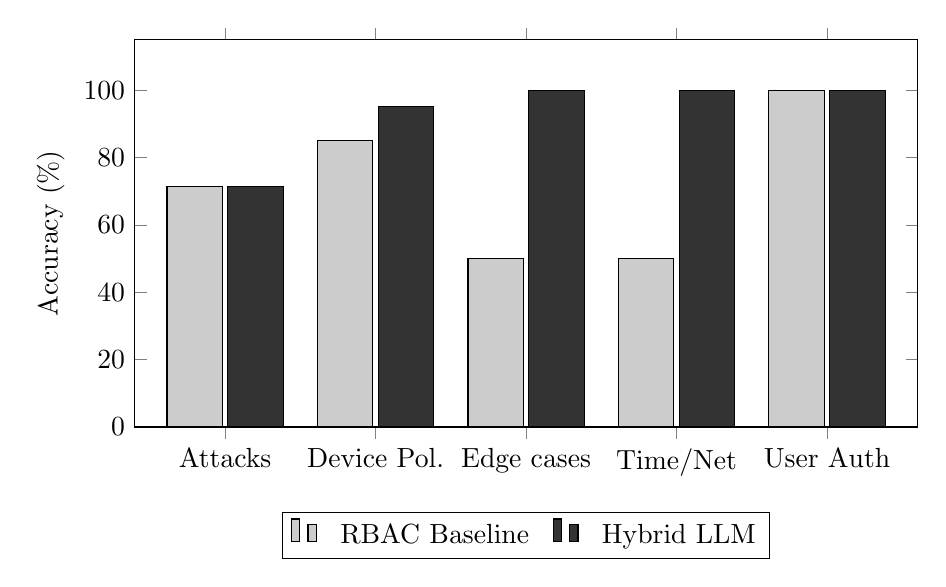
\begin{tikzpicture}
        \begin{axis}[
            ybar=2pt, % Added spacing between grouped bars to prevent overlap
            bar width=20pt,
            width=0.95\textwidth,
            height=6.5cm,
            enlarge x limits=0.15,
            legend style={
                at={(0.5,-0.22)}, % Lowered slightly to give breathing room from x-axis
                anchor=north, 
                legend columns=-1,
                column sep=1.5ex % Added horizontal spacing between legend items
            },
            ylabel={Accuracy (\%)},
            symbolic x coords={Attacks, Device Pol., Edge cases, Time/Net, User Auth},
            xtick=data,
            ymin=0, ymax=115, % Reduced ymax from 125 to 115 to reduce wasted top space
            ytick={0,20,40,60,80,100},
        ]
        % RBAC Baseline Data
        \addplot[fill=gray!40] coordinates {(Attacks,71.4) (Device Pol.,85.2) (Edge cases,50.0) (Time/Net,50.0) (User Auth,100.0)};
        
        % Hybrid LLM Data
        \addplot[fill=black!80, text=black] coordinates {(Attacks,71.4) (Device Pol.,95.1) (Edge cases,100.0) (Time/Net,100.0) (User Auth,100.0)};
        
        \legend{RBAC Baseline, Hybrid LLM}
        \end{axis}
    \end{tikzpicture}
    \caption{Category-wise performance comparison across the benchmark categories.}
    \label{fig:performance_chart}
\end{figure}

\textbf{User Authorization}: Both the hybrid system and the RBAC baseline achieved 100.0\% accuracy (20/20 correct) on the standardized user authorization test suite. This result is expected because deterministic validation in Layer 0 (user$\rightarrow$device permission matching) is conceptually shared with the RBAC baseline and applied before the LLM. The LLM semantic layer is not needed for this category, but it remains relevant for cases involving wildcard overlaps and ambiguous role-based delegations.

\textbf{Attack Detection and Vulnerability Mitigation}: Our red-team evaluation initially exposed vulnerabilities in LLM-based access control, where prompt injection bypassed naive semantic checks. With two-stage mitigation, the deterministic Layer 0 blocked 70 structural attacks (e.g., SQL injection, malformed IDs), and the sandboxed LLM layer denied the remaining 35 advanced semantic attacks. The result suggests that LLMs can support access authorization when robust input sanitization is employed.

\textbf{Time/Network and Device Policies}: Both systems performed similarly on deterministic time/network rules (87.5\% parity). The hybrid system performed better on device-specific policies (95.0\% vs. 85.0\%), which suggests that semantic metadata can improve performance when static rules are insufficient.

\subsection{Confidence Derivation and Post-Hoc Analysis}

Unlike standard classification models that rely on logit-based probabilities, IoT-Access-Sentinel logs Verbalized Semantic Confidence for auditing purposes. During the policy evaluation stage (Layer 2), the LLM agent is prompted to output a numerical confidence score ($c \in [0, 1]$) with its decision and reasoning. This score reflects the agent's semantic certainty with respect to the current policy context. While not used for live decision gating, these scores are recorded for post-hoc analysis and auditing. A key limitation is that LLM-generated text-based probabilities are often poorly calibrated, so verbalized confidence may not correlate well with empirical correctness unless formal calibration analysis is performed. We therefore analyze the confidence score as an ordinal metric rather than a runtime gating rule.

\subsection{Safety-Critical Metrics Analysis}\label{sec:safety_metrics}

Table~\ref{tab:safety_metrics} presents the precision, recall, and safety-critical error rates for both systems.

\begin{table}[h]
    \centering
    \caption{Safety Metrics: Precision, Recall, and Error Rates}
    \label{tab:safety_metrics}
    \begin{tabular}{lcc}
        \toprule
        \textbf{Metric}   & \textbf{RBAC Baseline} & \textbf{Hybrid LLM} \\
        \midrule
        \multicolumn{3}{l}{\textit{Performance Metrics}}                 \\
        Accuracy          & 82.4\%                 & \textbf{94.1\%}     \\
        Precision         & 78.7\%                 & \textbf{100.0\%}    \\
        Recall            & 82.2\%                 & \textbf{86.7\%}     \\
        \midrule
        \multicolumn{3}{l}{\textit{Safety-Critical Metrics}}             \\
        False Permit Rate & 17.5\%                 & \textbf{0.0\%}      \\
        False Deny Rate   & 17.8\%                 & \textbf{13.3\%}     \\
        \bottomrule
    \end{tabular}
\end{table}

\textbf{False Permit Rate (Security Breaches)}: The hybrid system produced no false permits in this benchmark (0.0\% vs 17.5\%). False permits correspond to unauthorized access attempts that bypass the control logic.

The system reliability was evaluated during a high-concurrency stress test. While the system maintained 100\% log-based security accuracy on successfully processed requests, we observed 34 API timeouts (24.8\% of the total requests) during peak load. Under our fail-secure policy, these timeouts defaulted to DENY, which shifts the balance toward security over availability during stress.


\subsection{Mitigation Performance: Semantic Caching}\label{sec:caching_results}
Our evaluation suggests that the Semantic Caching Layer (detailed in Section~\ref{sec:decision_pipeline}) can mitigate some availability concerns of remote LLMs. For repeated access requests, it bypasses inference and returns sub-millisecond responses, and it can serve cached decisions during cloud API outages.

\textbf{False Deny Rate and Fail-Secure Behavior}: The hybrid system defaults to DENY for API timeouts or internal pipeline failures. Although these fail-secure actions (34 instances out of 137 initiated requests) temporarily impact availability, they reduce the risk of unauthorized access during transient system instability. On the \textbf{102 completed scenarios} (204 total runs), all ``should-DENY'' requests were correctly blocked by the hybrid system, compared with 82.5\% for the RBAC baseline. In this setting, reduced availability does not necessarily imply weaker access control.

\textbf{Vulnerabilities and Mitigation in Red-Team Evaluation}: In our targeted red-team evaluation (Section~\ref{sec:adversarial_eval}, Table~\ref{tab:adversarial}) consisting of 105 high-intensity scenarios, initial LLM configurations failed against sophisticated prompt injection attacks. After the structural mitigations were added, the hybrid system handled all evaluated evasion attempts, indicating improved resistance once semantic bounds were enforced.

\textbf{Accuracy vs. Reliability}: The post-mitigation behavior reflects the system's structural reliance on the deterministic Layer 0 to filter malformed payloads, combined with strict LLM data bounding. This defense-in-depth approach supports reliability under adversarial conditions.

\subsection{System Performance Metrics}

Table~\ref{tab:performance} summarizes the runtime performance characteristics.

\begin{table}[h]
    \centering
    \caption{Runtime Performance and Resource Usage}
    \label{tab:performance}
    \begin{tabular}{lc}
        \toprule
        \textbf{Metric}                 & \textbf{Value} \\
        \midrule
        Avg. End-to-End Latency         & 97 ms          \\
        \quad Camera Scenarios          & 156 ms         \\
        \quad Sensor Scenarios          & 38 ms          \\
        \quad Deterministic-Only        & $<$1 ms        \\
        Throughput (5 concurrent)       & 31.5 RPS       \\
        Memory Usage                    & 94 MB          \\
        CPU Utilization                 & $<$1\%         \\
        LLM Calls Saved (Deterministic) & 46\%           \\
        API Success Rate                & 75.2\%         \\
        \bottomrule
    \end{tabular}
\end{table}

Latency breakdown shows that 46\% of requests are resolved in under 1ms via deterministic validation, whereas camera scenarios requiring full LLM context analysis average 156ms. Sensor scenarios, involving simpler policies, complete in 38ms. The 31.5 RPS throughput under concurrent load suggests the system can scale to enterprise deployments, and the low resource usage (94MB memory, $<$1\% CPU) indicates feasibility on modest hardware.

\section{Discussion}

\subsection{Agent Security and Authorization Boundaries}

To address the trust--authorization gap inherent in probabilistic agentic systems~\cite{nistai2024}, we define explicit authorization boundaries and tool-use scoping for the sentinel.

\textbf{Information Flow Control}: The multi-agent architecture uses a ``need-to-know'' data partitioning strategy. The \textit{Context Agent} receives raw network/device metadata to generate a situational report, whereas the \textit{Policy Agent} receives that report alongside the relevant security policies. This separation reduces the risk that a compromised agent can fabricate context for an unauthorized bypass.

\textbf{Tool-Use Scoping}: Unlike general-purpose autonomous agents, the sentinel does not expose open-ended tool-use privileges. The LLM agents operate within a ``read-only'' reasoning sandbox and can only generate a structured \texttt{EnforcementAction} (DENY, PERMIT, or ESCALATE). The actual action on the security infrastructure (for example, blocking an IP via Wazuh) is performed by a deterministic, non-LLM \textit{Enforcement Controller}. This separation limits the effect of prompt injection to the reasoning layer.

\textbf{Least-Privilege Reasoning}: The sentinel restricts the LLM's influence to the semantic resolution of existing policy conflicts. The agentic layer cannot create new policies or modify Layer 0 blocklists. Any LLM reasoning failures or internal processing errors default to a fail-secure DENY status.

\subsection{Governance and Systemic Risk Management}

Delegating runtime authorization to probabilistic LLM reasoning introduces risks that must be managed through governance and fallback mechanisms.

\textbf{Availability and Fallback}: To mitigate ``outage-induced false denies'' caused by API latency or service unavailability, the sentinel implements a \textit{Dual-Mode Fallback}. If the LLM agents fail to respond within a 150ms timeout, the system defaults to Layer 0 (Deterministic) enforcement. In this mode, ``unambiguous'' requests are still handled, while ``semantically complex'' requests are diverted to an \textbf{Escalation Queue} (fail-secure) for human review or cached-policy enforcement. This reduces dependence on cloud API reliability. The fail-secure design also introduces a Denial of Service (DoS) risk: given the observed 24.8\% API timeout rate defaulting to DENY during stress testing, an adversary could flood the system with complex semantic requests to induce timeouts and deny legitimate access. Future work should consider rate-limiting or localized small language models (SLMs) to mitigate this threat.

\textbf{Integrity and Governance}: To address integrity risks such as prompt injection or jailbreaking, the sentinel employs \textit{Semantic Guardrails} and mandatory \textit{Audit Trails}. Every agent reasoning step is logged as a ``Policy Explanation'' in the SIEM, allowing SOC operators to inspect hallucinated permits after the fact. A multi-agent ``consensus'' model provides an additional governance layer, where the Auditor Agent checks whether the Policy Agent's decision aligns with the provided policy context.

\textbf{Privacy and Data Sovereignty}: Sending sensitive IoT metadata (e.g., user IDs, geolocation) to third-party APIs creates a privacy cost. While our current evaluation uses cloud-based Groq inference, our architectural roadmap emphasizes \textbf{Local Differential Privacy (LDP)} and on-premise offloading. By identifying and redacting Personally Identifiable Information (PII) at layer 0 before it reaches the semantic layer, the sentinel reduces the data exposure surface.

\section{Limitations and Future Work}

\subsection{Real Device Deployment Considerations}

\subsubsection{Current Evaluation Scope}

Our evaluation uses \textbf{simulated Wazuh alerts} generated from synthetic scenarios. Although the decision pipeline and enforcement integration were implemented end-to-end, the alerts represent hypothetical IoT access attempts rather than live device traffic. The controlled setup enabled comprehensive adversarial testing (102 scenarios) and fair baseline comparison, but it limits claims about field deployment performance.

\subsubsection{Deployment Feasibility}

The Wazuh agent (ossec-agent) has relatively modest resource requirements, typically fitting within 8--32 MB of RAM, requiring only a small amount of storage, and operating over intermittent connectivity because logs are buffered locally~\cite{wazuh2024}. This suggests feasibility for many higher-end IoT devices, including smart cameras, industrial sensors, and edge gateways. In contrast, ultra-constrained devices such as Arduino-class boards or ESP8266 nodes would likely require gateway proxy deployment rather than direct agent installation.

\subsubsection{Enforcement Integration}

The system was integrated with the Wazuh Active Response API~\cite{wazuh2024} for distributed IP blocking, and testing was performed in a development environment using Docker containers to simulate IoT agents. A production rollout would still require firewall configuration for enforcement targets, authenticated manager connections, and explicit validation of fail-safe behavior under network partitions. For constrained environments, a reverse-proxy gateway running Wazuh agents remains a practical option because it centralizes enforcement while reducing per-device overhead.

\subsection{Dataset Realism and Generalization}

\subsubsection{Synthetic Dataset Justification}
The primary limitation of our current evaluation is the reliance on a synthetic dataset (102 scenarios) derived from policy author assumptions. We chose this design to control the evaluation conditions for the semantic reasoning layer. Public datasets such as UNSW-NB15 or IoT-Dev-2024, while ecologically valid for network patterns, lack fine-grained semantic metadata and ``policy-ground truth'' labels (e.g., M0801-specific authorization conflicts) required to benchmark LLM reasoning depth. Using author-defined labels, we isolated the sentinel's ability to align complex natural language intent with defined security policies, which is a prerequisite for assessing generalizability before field deployment.

\subsubsection{Generalization and Distribution Shift}
A significant open question is how the system generalizes to cross-site environments or shifts in device behavior distributions. Our current evaluation assumes a static relationship between the user roles and device metadata, whereas these relationships are dynamic in real-world operator workflows. We acknowledge that the LLM's semantic reasoning may exhibit a distribution shift when encountering novel device types that are not included in our categorical definitions.

\subsubsection{Roadmap for Real-World Validation}
To address the lack of ecological validity in this pilot study, future work should emphasize cross-dataset validation against real-world traces, a human-in-the-loop study in which SOC analysts assess LLM-generated reasoning, and high-fidelity testbed deployment in office or industrial environments. Together, these steps would help determine whether the current results generalize beyond author-defined ground truth.

\subsection{Additional Limitations}

The current evaluation remains limited in three respects. First, it was run with a single LLM model (Llama 3.1 8B via Groq), so performance may differ for other models. Second, the system depends on an external API, and the observed rate-limiting failures show that a local model or caching layer would be needed for more robust deployment. Third, the benchmark covers access-control policies only; firmware updates, encryption, and other IoT security concerns were outside the scope of the present study.

\textbf{Artifact Availability}: Benchmark scenarios, system prompts, and baseline implementations are publicly available at \texttt{https://github.com/ahmed-fouad-lagha/IoT-Access-Sentinel} to facilitate reproduction and extension of this work.

\subsection{Future Research Directions}

Although our hybrid architecture shows that zero-shot general-purpose LLMs can support IoT access control, several avenues warrant further investigation.

\subsubsection{Domain-Specific LLM Fine-Tuning}

The current system uses a pretrained general-purpose model (Llama 3.1 8B)~\cite{touvron2023llama}, which offers broad generalizability but also introduces API costs and latency. Fine-tuning smaller domain-specific models, such as 1B--3B parameter variants, on IoT-specific threat patterns could reduce latency, lower operating cost, improve privacy by eliminating external API dependence, and potentially improve detection of device impersonation, semantic policy evasion, and time-based bypasses. A next step is to benchmark such models against a semantic rule engine, for example OPA/Rego augmented with graph-based context retrieval, to compare shallow rule-based reasoning with LLM-based semantic reasoning. Open questions remain about the amount and balance of labeled data needed, whether a 7B fine-tuned model can approach GPT-4-class accuracy, and how model size affects the latency-accuracy trade-off in production deployments. Achieving this would likely require on the order of 10,000 labeled IoT access scenarios covering multiple device types, policy violations, and representative attacks.

\subsubsection{Feasibility Analysis: Edge Offloading and Model Compression}

To reduce the latency and cost overhead of cloud-based APIs, we also examined local inference through model compression. Quantizing Llama-3-8B~\cite{llama3} to 4-bit integer precision substantially lowers memory requirements and makes deployment on edge hardware more realistic, although some accuracy loss is expected. On-device inference is still slower than the current Groq-based implementation~\cite{groq2024}, but it may be acceptable for reactive blocking when Layer 0 continues to provide immediate fail-secure protection. In this setting, local inference improves data sovereignty and cloud independence while keeping the semantic layer available for deeper analysis.

\subsubsection{Architectural Hybridization: Semantic Leases}

A further direction is to combine runtime reasoning with CollabIoT-style formal token models through Semantic Leases. In this design, the agentic sentinel would generate short-lived machine-enforceable access tokens that encode semantic predicates rather than rigid identities, while a lightweight edge controller would perform the actual enforcement. This approach could preserve semantic oversight while removing the LLM from the high-frequency enforcement path.

\subsubsection{Reproducibility and Open-Source Artifacts}

The source code, benchmark scenarios, prompt templates, and reproduction scripts for IoT-Access-Sentinel are available in the project repository.

\section{Conclusion}

We present IoT-Access-Sentinel, a hybrid multi-agent framework for IoT access control that combines deterministic authorization with LLM-based contextual reasoning. Our evaluation highlights the security trade-offs of this design. Initial testing showed that the LLM reasoning layers were vulnerable to prompt injection. After adding deterministic containment and strict data delimiters, the system handled the benchmarked attacks more robustly. By integrating with the Wazuh SIEM ecosystem, Sentinel offers one possible design for security teams. The study suggests that future agentic IoT security should prioritize adversarial resilience alongside semantic flexibility.

\begin{acknowledgments}
This research was supported by the Eötvös Loránd University. We thank the Wazuh~\cite{wazuh2024} and Groq~\cite{groq2024} teams for their open-source tools and accessible AI infrastructure based on Llama models~\cite{touvron2023llama}.
\end{acknowledgments}

\section*{Declaration on Generative AI}
During the preparation of this work, the author(s) used Llama 3.1 and Groq to run access control evaluation scenarios and generate decision metrics as part of the experimental framework. Furthermore, generative AI was used for proofreading and grammatical refinement of the manuscript. After using these tool(s)/service(s), the author(s) reviewed and edited the content as needed and took full responsibility for the publication’s content.

\bibliography{references}

\end{document}
